\section{GLSL Phong Source Code}
\label{app:llphong}

This section lists the full code for the Phong lighting model in plain GLSL~\cite{glsl}.

\begin{verbatim}
	precision mediump float;
	
	// External Function Declarations
	uniform mat4 uModel;
	uniform mat4 uView;
	varying vec3 vNormal;
	uniform vec3 uLight;
	varying vec3 vPosition;
	
	void main() {
		vec3 ambient = vec3(.1, 0., 0.);
		vec3 lightColor = vec3(0.4, 0.3, 0.9);
		vec3 specColor = vec3(1., 1., 1.);
		
		vec4 homWorldPos = uModel*vec4(vPosition, 1.0);
		vec3 camPos = normalize(vec3(uView*homWorldPos));
		vec3 worldNorm = 
		normalize(vec3(uModel*vec4(vNormal, 0.0)));
		
		vec3 lightDir = 
		normalize(uLight - vec3(homWorldPos));
		vec3 reflectDir = reflect(lightDir, worldNorm);
		
		vec3 diffuse = 
		max(lightWorldDot, 0.0) * lightColor;
		
		float spec = pow(max(-dot(
		camPos, reflectDir), 0.), 32.);
		vec3 specular = spec * specColor;
		
		gl_FragColor = vec4(ambient+diffuse+specular, 1.0);
	}
\end{verbatim}

\section{Gator Phong Source Code}
\label{app:hlphong}

This section lists equivalent code in Gator.

\begin{verbatim}
	#"precision mediump float;";
	using "../glsl_defs.lgl";
	
	// Reference Frame Declarations
	
	frame model has dimension 3;
	frame world has dimension 3;
	frame camera has dimension 3;
	frame light has dimension 3;
	
	// Global Variables
	
	varying cart3<model>.point vPosition;
	canon uniform hom<model>.transformation<world> uModel;
	canon uniform hom<world>.transformation<camera> uView;
	varying cart3<model>.vector vNormal;
	uniform cart3<light>.point uLight;
	canon uniform hom<light>.transformation<world> uLightTrans;
	
	// Shader Code
	
	void main() {
		color ambient = [.1, 0., 0.];
		color diffColor = [0.4, 0.3, 0.9];
		color specColor = [1.0, 1.0, 1.0];
		
		auto worldPos = vPosition in world;
		auto camPos = worldPos in camera;
		auto worldNorm = normalize(vNormal in world);
		
		auto lightDir = normalize((uLight in world) - worldPos);
		auto lightWorldDot = dot(lightDir, worldNorm);
		scalar diffuse = max(lightWorldDot, 0.0);
		
		auto reflectDir = normalize(reflect(-lightDir, worldNorm) in camera);
		
		scalar specular = pow(max(dot(normalize(-camPos), reflectDir), 0.), 32.);
		
		vec4 gl_FragColor = 
		vec4(ambient + diffuse * diffColor + specular * specColor, 1.0);
	}
\end{verbatim}

\section{Case Study Images}

\begin{figure}
	\centering
	\begin{subfigure}[b]{0.45\linewidth}
		\centering
		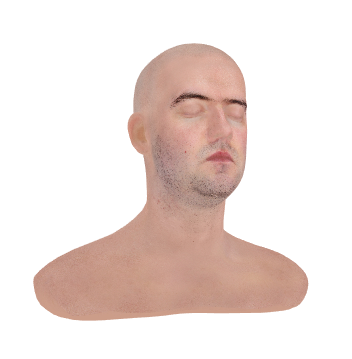
\includegraphics[width=\linewidth]{fig/texture.png}
		\caption{Texture.}
	\end{subfigure}
	\hfill
	\begin{subfigure}[b]{0.45\linewidth}
		\centering
		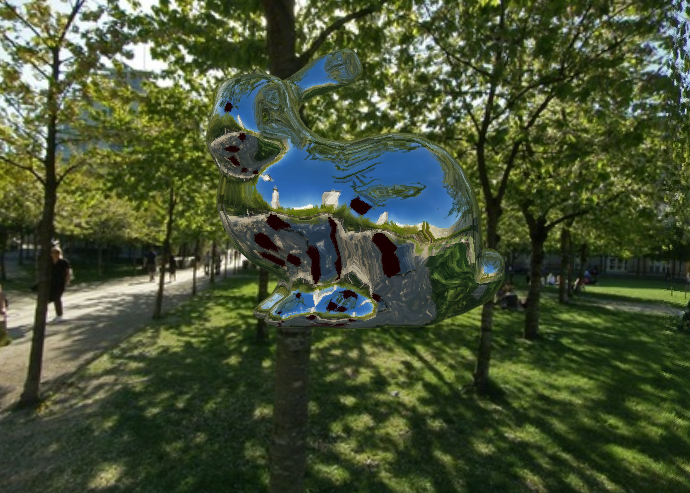
\includegraphics[width=\linewidth]{fig/reflection.png}
		\caption{Reflection.}
	\end{subfigure}
	
	\begin{subfigure}[b]{0.45\linewidth}
		\centering
		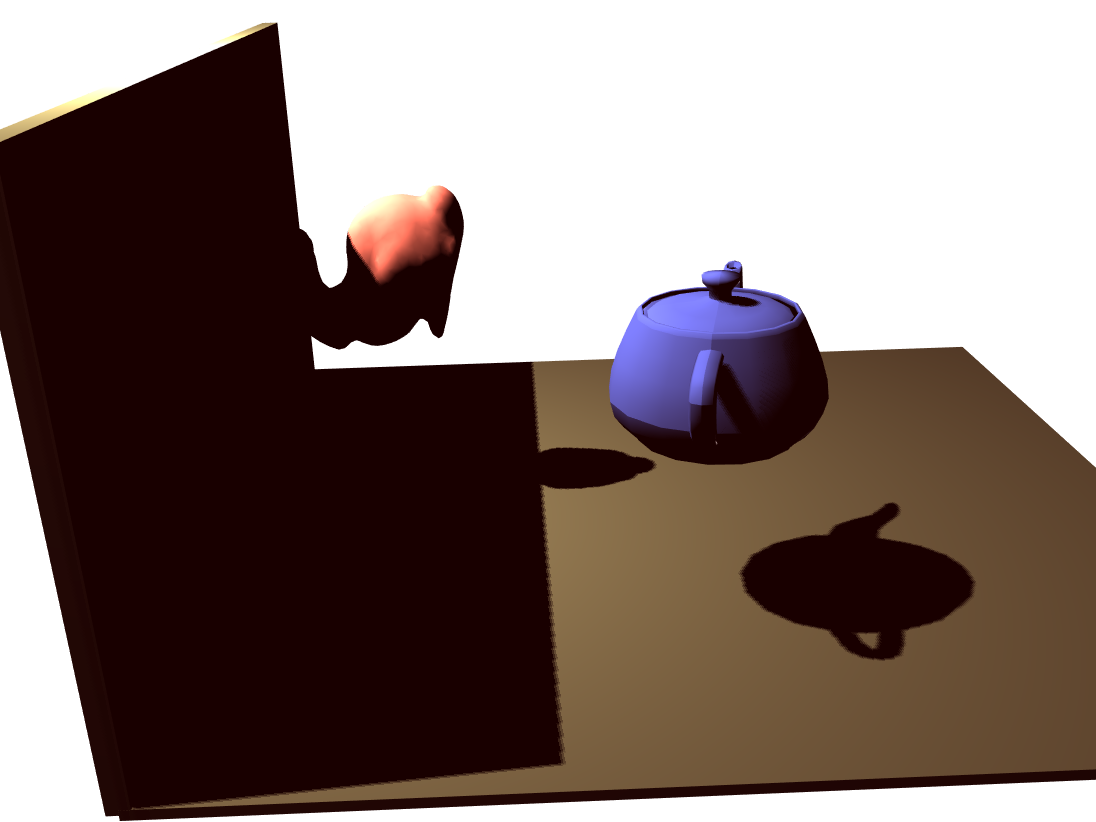
\includegraphics[width=\linewidth]{fig/shadowmap.png}
		\caption{Shadow map.}
	\end{subfigure}
	\hfill
	\begin{subfigure}[b]{0.45\linewidth}
		\centering
		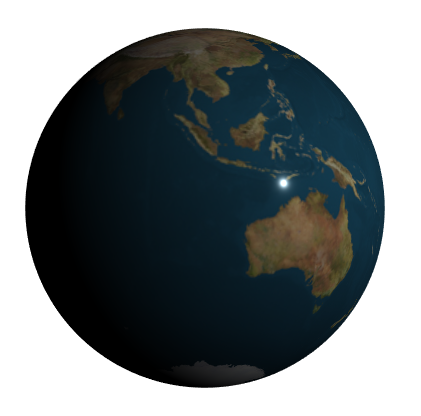
\includegraphics[width=\linewidth]{fig/microfacet.png}
		\caption{Microfacet.}
	\end{subfigure}
	\caption{Example outputs from first four renderers used in our case studies.}
\end{figure}
\begin{figure}
	\begin{subfigure}[b]{0.45\linewidth}
		\centering
		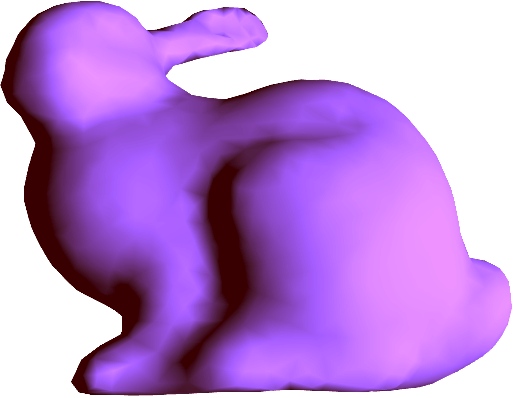
\includegraphics[width=\linewidth]{fig/bunnygoodfront.png}
		\caption{Phong}
	\end{subfigure}
	\hfill
	\begin{subfigure}[b]{0.45\linewidth}
		\centering
		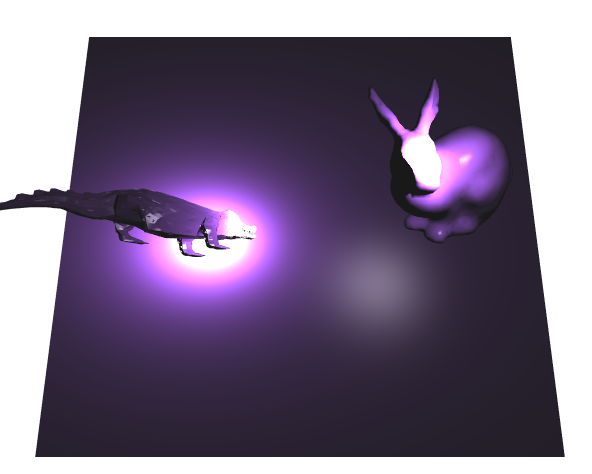
\includegraphics[width=\linewidth]{fig/fog.png}
		\caption{Fog}
	\end{subfigure}
	\begin{subfigure}[b]{0.45\linewidth}
		\centering
		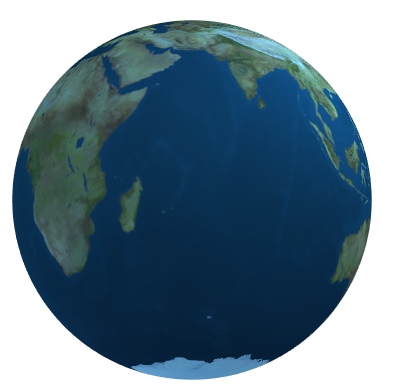
\includegraphics[width=\linewidth]{fig/bump.png}
		\caption{Bump Map}
	\end{subfigure}
	\hfill
	\begin{subfigure}[b]{0.45\linewidth}
		\centering
		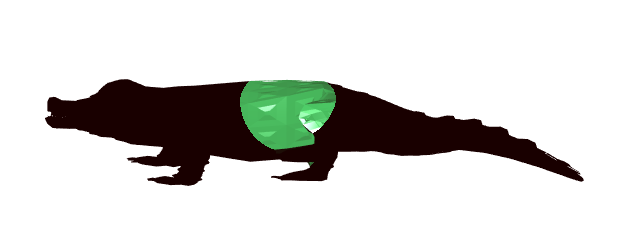
\includegraphics[width=\linewidth]{fig/spotlight.png}
		\caption{Spotlight}
	\end{subfigure}
	\caption{Example outputs from last four renderers used in our case studies.}
\end{figure}